% Preamble
\documentclass[11pt,a4paper]{article}
\usepackage{amsmath,amssymb,amsfonts,amsthm}
\usepackage{graphicx}
\usepackage{wrapfig}
\usepackage[a4paper]{geometry}
\usepackage{caption}
\usepackage{lscape}
\usepackage{array}
\usepackage{subcaption}
\usepackage{grffile}
\usepackage{rotating}
\usepackage[pdfborder={0 0 0}]{hyperref}
\usepackage[section] {placeins}
\newcommand{\field}[1]{\mathbb{#1}}  % the font for a mathematical field is blackboard
\newcommand{\R}{\field{R}} % the field of the reals
\newcommand{\N}{\field{N}} % the field of the natural numbers
\newcommand{\C}{\field{C}} % the field of complex number
\newcommand{\Z}{\field{Z}} % the field of integers
\theoremstyle{plain}
  \newtheorem{stelling}{Stelling}
  \newtheorem{lemma}[stelling]{Lemma}
  \newtheorem{gevolg}[stelling]{Gevolg}
\theoremstyle{definition}
  \newtheorem{definitie}[stelling]{Definitie}
  \newtheorem{voorbeeld}[stelling]{Voorbeeld}
\theoremstyle{remark}
  \newtheorem*{noot}{Noot}
  
\newcommand{\drsh}{\reflectbox{\rotatebox[origin=c]{180}{\Huge $\Rsh$ \hspace{3pt}}}}

\textheight 230truemm
  
\begin{document}
\begin{center}
{\huge {\tt CRADLE++} Documentation}
\vspace{20pt}

{\large Customisable RAdioactive Decay for Low Energy Particle Physics: \\ A C++ event generator}
\vspace{15pt}

{\small \href{mailto:leendert.hayen@fys.kuleuven.be}{leendert.hayen@fys.kuleuven.be}}
\vspace{10pt}

\today
\end{center}

\section{Introduction}
This C++ package attempts to provide a general event generator for low energy particle physics, specifically nuclear spectroscopy studies. Its main focus lies on weak interaction studies perpetuated by nuclear beta decay. Its goals are accessibility and extendibility.
\\ \\
The general structure of the cradle CRADLE++ program is as follows

\begin{tabbing}
DecayManager: \= Performs the main loop, keeps the particle stack, particle factory \\ \> and the registered DecayModes.
\end{tabbing}
\begin{tabbing}
\hspace{10pt}
\drsh Particle: \= Contains physical information (mass, charge, \ldots), kinematical \\ \> information, and array of DecayChannels.
\end{tabbing}
\begin{tabbing}
\hspace{20pt}
\drsh DecayChannel: \= Contains intensity, parent and daughter excitation energy,\\ \> Q value, lifetime and DecayMode.
\end{tabbing}
\begin{tabbing}
\hspace{30pt}
\drsh DecayMode: \= Dynamics of the specific decay. Inherited by daughter\\ \> classes BetaMinus, Alpha, etc. Parent class performs\\ \> TwoBodyDecay() and ThreeBodyDecay(), daughter\\ \> classes perform particle creation and initialisation.
\end{tabbing}
\section{Prerequisites}
We attempted to use as few external libraries as possible without slowing down the coding progress. Two libraries were used. Both are extensive and widespread C++ libraries, typically installed by default on Linux systems.
\begin{enumerate}
\item BOOST: The linear algebra routines of uBLAS, and the program\_options library are extensively used. (\url{http://www.boost.org})
\item Gnu Scientific Library (GSL): Used for the calculation of the calculation of the complex Gamma function in the Fermi function. (\url{http://www.gnu.org/software/gsl/})
\end{enumerate}
 When using the precompiled binary, the libraries are statically included, and require only a Linux 64-bit system to run. Building requires the boost libraries to be installed, if not done already. This can be done easily using the package manager {\tt sudo apt-get install libboost-dev} (replace {\tt apt-get} for any other package manager on your system).
\vspace{10pt}

CRADLE++ uses the data files from NNDC and ENSDF databases, as compiled for the Geant4 distribution. These can be downloaded at \url{http://geant4.web.cern.ch/geant4/support/download.shtml}. CRADLE++ uses the G4RadioactiveDecayX.X and G4PhotonEvaporationX.X data files.
\vspace{10pt}

CRADLE++ was tested on Ubuntu 14.04 LTS, and Ubuntu 15.10 in a fresh virtual machine install.

\section{Configuration}
All options can be seen by running the program with the -h [--help] flags.
\vspace{10pt}

CRADLE++ requires a configuration file on start-up to set several parameters, such as weak interaction coupling constants, general verbosity or lifetime cuts. Options are written in typical INI format. By default {\tt config.txt} in the local folder is loaded. This behaviour can be overridden using command line options.
\vspace{10pt}

The location of the data files can be set using the environment variables CRADLE\_GammaData and CRADLE\_RadiationData. In case these are not defined, CRADLE++ looks for them in the GammaData and RadiationData local folders.

\section{Usage}
CRADLE++ performs the full decay chain until it arrives at a state with a lifetime longer than the value {\tt Cut.Lifetime} in seconds specified in the configuration file. It starts from an initial state with a name, Z value, A value and an excitation energy. The initial state is at rest. Beta decay is currently the only DecayMode where angular correlations have been implemented. Each decay is performed in the rest frame of the mother and afterwards Lorentz boosted into the lab frame. In the calculation natural units are used, i.e. $\hbar=c=m_e=1$. The standard energy scale is keV. Output is by default written to {\tt output.txt}. This behaviour can be overridden with the command line options.
\vspace{10pt}

The structure of the output file is as follows:
\begin{itemize}
\item Column 1: Event ID
\item Column 2: Time of particle creation in seconds. The decay of the parent is included.
\item Column 3: Particle name
\item Column 4: Excitation energy
\item Column 5: Kinetic energy (keV)
\item Column 6-9: Four momentum of emitted particle in lab frame
\end{itemize}
Particles are emitted in a $4\pi$ solid angle and momentum conservation is guaranteed.

\section{Example}
We study the proton spectrum after emission from $^{32}$Cl($E_{X}=5046.3$\,keV) after $\beta^+$ decay from $^{32}$Ar for both scalar and vector interactions. Setting {\tt Couplings.CS} and {\tt Couplings.CV} to 0 and 1 in {\tt config.txt}, respectively, we run CRADLE++ as follows
\vspace{10pt}

{\tt ./Cradle++ -n 32Ar -z 18 -a 32 -l 500000 -f 32Ar\_vector.txt}
\vspace{10pt}

Doing the same thing, but reversing the two coupling constants we get the scalar recoil spectrum. Both are plotted in figure \ref{fig:32Ar_p}. The gamma rays from the decay are shown in figure \ref{fig:32Cl_gamma}. 
\vspace{10pt}

\textbf{Note}: This is a special case, as nucleon emission is not included in the Geant4 codebase, and so it is not present in its data files. It can however be added manually without any issue. See the README file of the G4RadioactiveDecayX.X for the structure of the data files. Proton decay can then be trivially included by adding

\begin{verbatim}
# Denotes metastable state; Excitation Energy; Lifetime
P       5046.3          0.0000e+00
# Decay modes from this state; Name; Daughter Excitation; Intensity; Q
                      Proton  0.0000e+00      1.0000e+02      3.4580e+03
\end{verbatim}
to the data file {\tt z17.a32}. The intensity (here set to $J_p = 100.0$) is used to choose the decay mode via the probability
\begin{equation}
P(p) = \frac{J_p}{\sum_i J_i}
\end{equation}
where $J_i$ denotes the intensity of the $i$-th decay channel from the current state. This means it competes with $\gamma$ decay from the same level. Isolating the proton emission can be done simply by increasing $J_p$.
\begin{figure}[h!]
\vspace{-20pt}
\centering
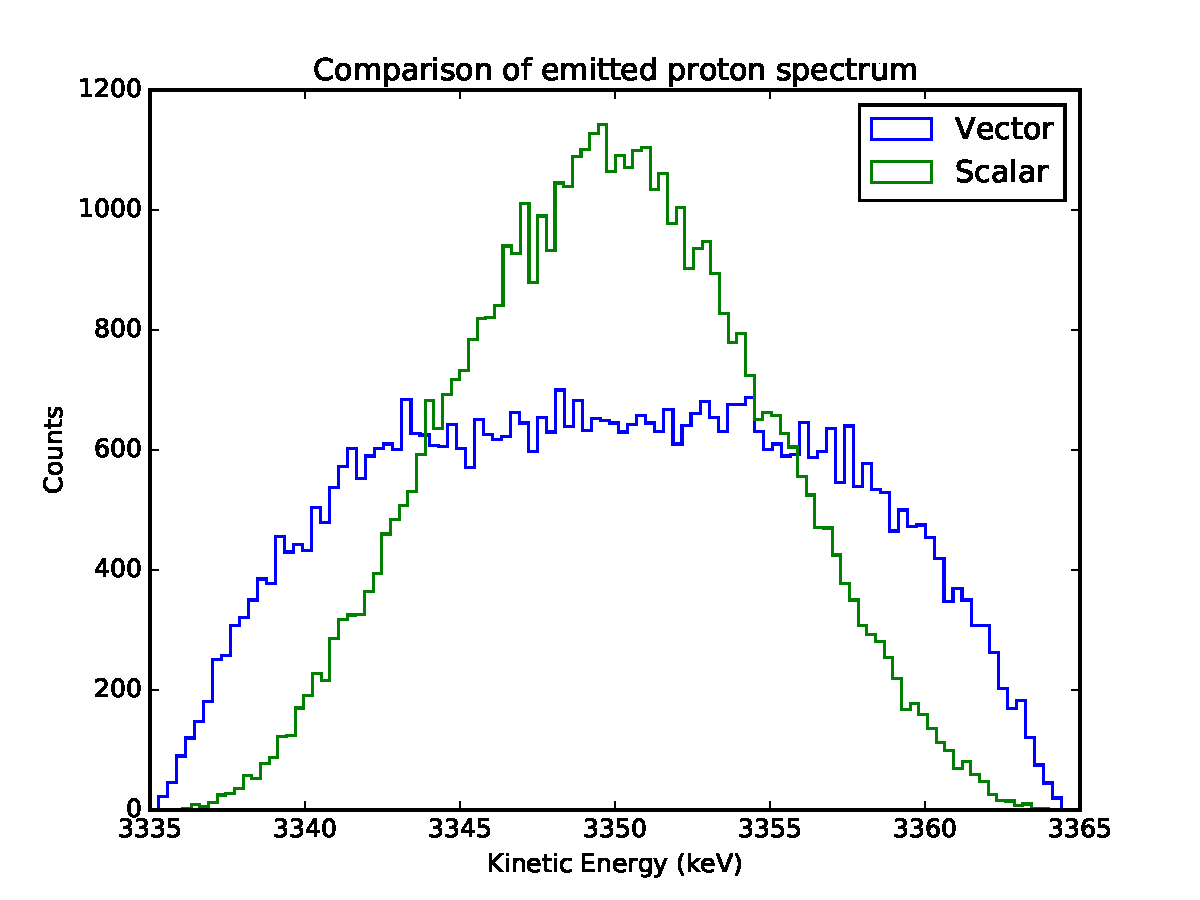
\includegraphics[width=\textwidth]{32Ar_proton.pdf}
\caption{Comparison of the proton peak after emission from $^{32}$Cl for a vector and scalar interaction.}
\label{fig:32Ar_p}
\end{figure}

\begin{figure}[h!]
\vspace{-30pt}
\centering
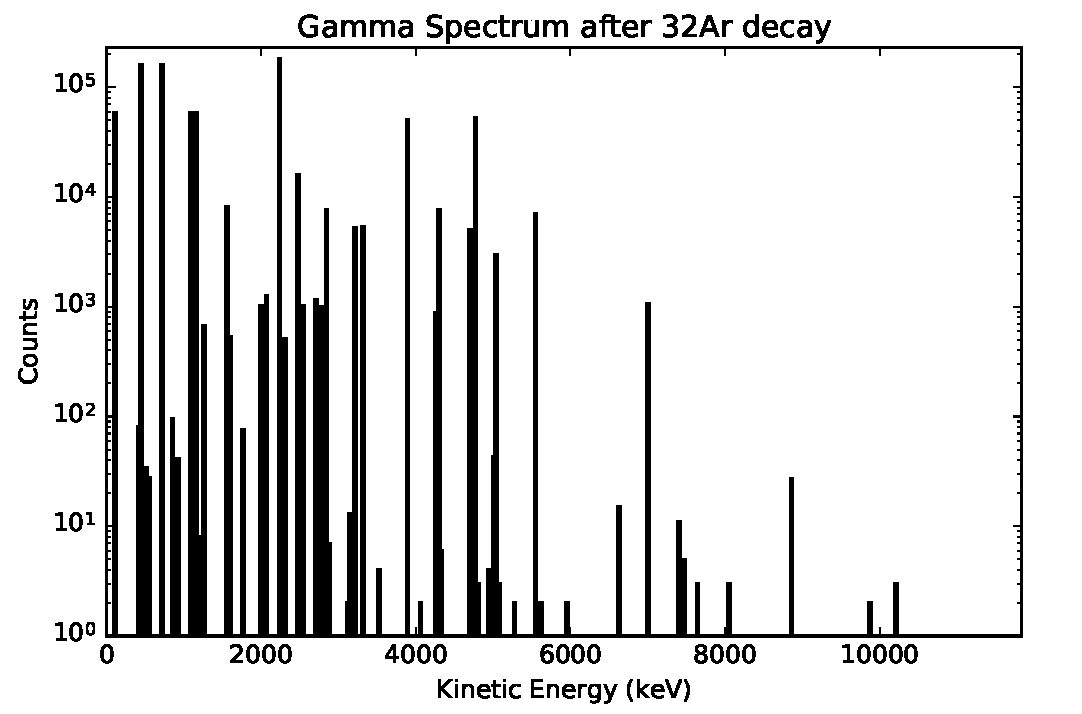
\includegraphics[width=0.95\textwidth]{32Ar_gamma.pdf}
\caption{Gamma spectrum after $\beta^+$ decay of $^{32}$Ar. The highest $\gamma$ energies above 10\,MeV come from very weakly populated levels in $^{32}$P after $\beta^+$ from $^{32}$Cl.}
\label{fig:32Cl_gamma}
\end{figure}
\end{document}
